\documentclass{article}
\usepackage[utf8]{inputenc}
\usepackage[dutch]{babel}
\usepackage[square,sort,comma,numbers]{natbib}
\usepackage[hyphens]{url}
\usepackage{tikz}
\usetikzlibrary{trees}
\usepackage{float}
\usepackage{hyperref}
\setlength
{\parindent}
{0pt}
\setlength
{\parskip}
{1.5ex plus 0.5ex minus 0.2ex}
\usepackage[margin=3.5cm]{geometry}


\title{Artificiële Intelligentie: Opdracht 1 (Version Spaces)}
\author{Mathias Van Herreweghe - r0456156}
\date{21 november 2014}

\usepackage{natbib}
\usepackage{graphicx}

\begin{document}

\maketitle
\newpage

\section{Opgave}
Je bent rustig door het Arenberg park aan het wandelen langs de voetbalvelden om diep na te denken over een complex algoritme. Plots komt er een weelderige dame in voetbaltenue jouw hulp vragen, ze ziet direct dat je een informaticus bent. Ze vertelt dat ze coach is van een damesploeg van de KU Leuven. Ze zoekt naar enkele nieuwe spitsen om haar team uit te breiden. Ze vraagt of jij een systeem wil uitwerken dat interessante spitsen filtert uit de honderden inzendingen die ze heeft ontvangen. Uiteraard zeg je toe.

De coach vraagt aan de kandidaten om enkele belangrijke eigenschappen in te vullen. De meest specifieke eigenschappen die men kan invullen worden hieronder weergegeven.

\begin{itemize}
\item Voorkeur voet: links - rechts
\item Gewicht: licht - gemiddeld - zwaar
\item Specialiteit: sprint - counter-aanval - precisie-schot - kracht-schot
\item Hobby: partner - uitgaan - fitness - basketbal - zwemmen - schaken
\end{itemize}

Verder heeft de coach de eerste 6 ontvangen inzendingen beoordeeld, deze beoordelingen vind je in Tabel \ref{beoordeling}.

\begin{table}[H]
\centering
\begin{tabular}{ c | c | c | c | c | c}
\hline
 \# & positie & gewicht & specialiteit & hobby \\
  \hline
 1 & links & gemiddeld & sprint & basketbal & + \\
 2 & links & zwaar & kracht-schot & uitgaan & - \\
 3 & rechts & licht & sprint & partner & - \\
 4 & rechts & gemiddeld & counter-aanval  & fitness & + \\
 5 & links & gemiddeld & sprint & schaken & + \\
 6 & rechts & gemiddeld & precisie-schot & schaken & - \\
  \hline
\end{tabular}
\caption{Beoordeling}
\label{beoordeling}
\end{table}

Na het gesprek komt er een dame zich spontaan aanmelden bij de coach, ze zegt linksvoetig te zijn, een licht gewicht hebben, zwemmen als hobby hebben en haar specialiteit is een counter-aanval.

Het is nu aan jou om een systeem uit te werken, gebruik makend van de gegeven test-data, aan de hand van Version Spaces om na te gaan of deze dame het tot het team zal maken.

\begin{figure}[H]
\centering
\caption{Hypothesetaal}
\label{hypothesetaal}
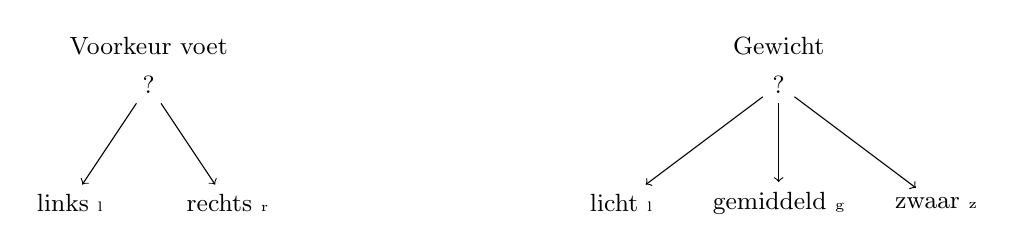
\begin{tikzpicture}
\node (v) at (-4,-0.5) {\small Voorkeur voet};
\node (vi) at (-4,-1) {\small ?};
\node (vA) at (-5,-2.5) {\small links \tiny l};
\node (vB) at (-3,-2.5) {\small rechts \tiny r};
\draw[->] (vi) -- (vA);
\draw[->] (vi) -- (vB);

\node (g) at (4,-0.5) {\small Gewicht};
\node (gi) at (4,-1) {\small ?};
\node (gA) at (2,-2.5) {\small licht \tiny l};
\node (gB) at (4,-2.5) {\small gemiddeld \tiny g};
\node (gC) at (6,-2.5) {\small zwaar \tiny z};
\draw[->] (gi) -- (gA);
\draw[->] (gi) -- (gB);
\draw[->] (gi) -- (gC);
\end{tikzpicture}\\\vspace{0.5cm}
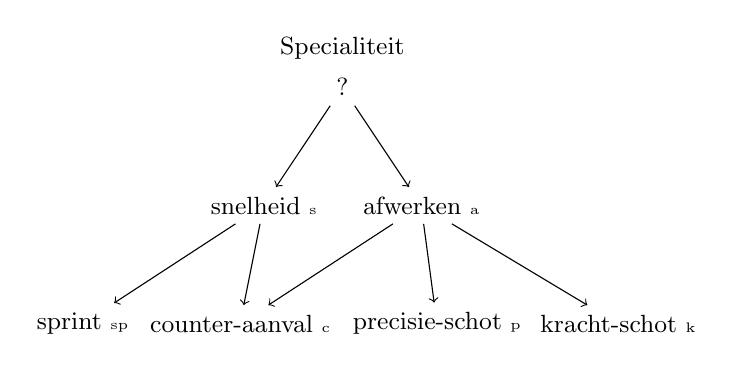
\begin{tikzpicture}
\node (s) at (0,-0.5) {\small Specialiteit};
\node (si) at (0,-1) {\small ?};
\node (sA) at (-1,-2.5) {\small snelheid \tiny s};
\node (sB) at (1,-2.5) {\small afwerken \tiny a};
\draw[->] (si) -- (sA);
\draw[->] (si) -- (sB);
\node (sAa) at (-3.3,-4) {\small sprint \tiny sp};
\node (sAb) at (-1.3,-4) {\small counter-aanval \tiny c};
\draw[->] (sA) -- (sAa);
\draw[->] (sA) -- (sAb);
\node (sBa) at (1.2,-4) {\small precisie-schot \tiny p};
\node (sBb) at (3.5,-4) {\small kracht-schot \tiny k};
\draw[->] (sB) -- (sAb);
\draw[->] (sB) -- (sBa);
\draw[->] (sB) -- (sBb);
\end{tikzpicture}\\\vspace{0.5cm}
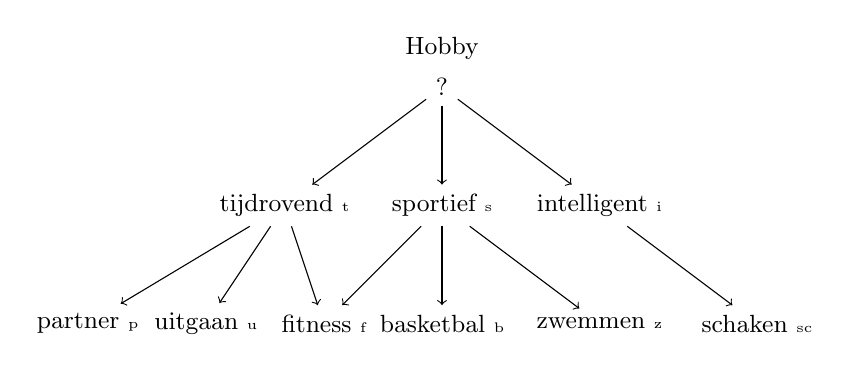
\begin{tikzpicture}
\node (h) at (-4,-0.5) {\small Hobby};
\node (hi) at (-4,-1) {\small ?};
\node (hA) at (-6,-2.5) {\small tijdrovend \tiny t};
\node (hB) at (-4,-2.5) {\small sportief \tiny s};
\node (hC) at (-2,-2.5) {\small intelligent \tiny i};
\draw[->] (hi) -- (hA);
\draw[->] (hi) -- (hB);
\draw[->] (hi) -- (hC);
\node (hAa) at (-8.5,-4) {\small partner \tiny p};
\node (hAb) at (-7,-4) {\small uitgaan \tiny u};
\node (hAc) at (-5.5,-4) {\small fitness \tiny f};
\draw[->] (hA) -- (hAa);
\draw[->] (hA) -- (hAb);
\draw[->] (hA) -- (hAc);
\node (hBa) at (-4,-4) {\small basketbal \tiny b};
\node (hBb) at (-2,-4) {\small zwemmen \tiny z};
\draw[->] (hB) -- (hAc);
\draw[->] (hB) -- (hBa);
\draw[->] (hB) -- (hBb);
\node (hCa) at (0, -4) {\small schaken \tiny sc};
\draw[->] (hC) -- (hCa);
\end{tikzpicture}
\end{figure}

\newpage
\section{Model oplossing}
Men voert het Version-Spaces algoritme uit aan de hand van de gegeven test-data. Ten eerste initialiseert men $S$ en $G$. $G$ is de meest algemene hypothese mogelijk en is dus consistent met alles, $S$ daarentegen is inconsistent met alles.
\[ G = \{[?,?,?,?]\} \]
\[ S = \{\bot\} \]

De hypothesen in $G$ en $S$ worden afgebeeld in een grafe, bij elke iteratie. Elke hypothese in het rood omlijnd is ongeldig en behoort niet meer tot $G$ of $S$ op het einde van de betreffende iteratie. De vorm van het rode knooppunt duidt aan waarom een bepaalde hypothese verwijderd is. De verschillende mogelijkheden zie je hieronder in Tabel \ref{tbl_legende}.

\begin{table}[H]
\centering
\begin{tabular}{| c | p{10cm} |}
\hline
 \raisebox{-1\height}{\includegraphics[scale=0.5]{nodes/node1.jpg}}& De hypothese is geen generalisatie (bij negatief voorbeeld), of specialisatie (bij positief voorbeeld) van minstens 1 hypothese van respectievelijk $S$ of $G$. \\ \hline
\raisebox{-0.3\height}{\includegraphics[scale=0.5]{nodes/node2.jpg}}& De hypothese is redundant aan een andere hypothese. \\ \hline
\raisebox{-0.7\height}{\includegraphics[scale=0.5]{nodes/node3.jpg}} & De hypothese schat het huidige voorbeeld incorrect in. Namelijk negatief bij een positief voorbeeld en vice versa. $\rightarrow$ pruning \\ \hline
\end{tabular}
\caption{Tabel dienend als legende voor grafen}
\label{tbl_legende}
\end{table}

Hieronder zie je de initiële toestand van de grafe.

\begin{figure}[H]
\centering
\caption{Initiële toestand}
\label{initial}
\includegraphics[scale=0.5]{iteration_graphs/initial.jpg}
\end{figure}

\newpage

\subsection{Iteratie 1}
Het eerste voorbeeld is positief. Men zal dus alle hypothesen in $S$ waaraan het voorbeeld negatief door wordt beoordeeld, minimaal moeten generaliseren tot het correct wordt ingeschat. Bij deze iteratie is de nieuwe hypothese in $S$ dus de hypothese die exact gelijk is aan het voorbeeld.

\begin{itemize}
\item $G = \{[?,?,?,?]\}$
\item $S = \{[l,g,sp,b]\}$
\end{itemize}

\begin{figure}[H]
\centering
\caption{Iteratie 1}
\label{iteratie1}
\includegraphics[scale=0.5]{iteration_graphs/iteration1.jpg}
\end{figure}

\subsection{Iteratie 2}
Het tweede voorbeeld is negatief. Men zal dus alle hypothesen in G die het voorbeeld positief inschatten minimaal moeten specificeren tot het het huidige voorbeeld negatief zal beoordelen. Er zijn verschillende mogelijkheden. Enkele ervan zullen worden verwijderd aangezien ze geen generalisatie zijn van minstens 1 hypothese van $S$. Dit is te zien op Figuur \ref{iteratie2}.

\begin{itemize}
\item $G = \{[?,g,?,?],[?,?,s,?],[?,?,?,s]\}$
\item $S = \{[l,g,sp,b]\}$
\item $Niet$ $toegevoegd$ $= \{[r,?,?,?],[?,l,?,?],[?,?,?,i]\}$
\end{itemize}

\begin{figure}[H]
\centering
\caption{Iteratie 2}
\label{iteratie2}
\includegraphics[scale=0.5]{iteration_graphs/iteration2.jpg}
\end{figure}

\subsection{Iteratie 3}
Het derde voorbeeld is opnieuw negatief. We herhalen dus de aanpak zoals in iteratie 2. Zo bekomen we de grafe zoals op Figuur \ref{iteratie3}. We moeten opnieuw enkele hypothesen verwijderen omdat deze geen generalisatie zijn van minstens 1 hypothese in $S$. Ook verwijderen we 2 mogelijkheden omdat deze redundant zijn.

\begin{itemize}
\item $G = \{[?,g,?,?],[?,?,?,s],[l,?,s,?]\}$
\item $S = \{[l,g,sp,b]\}$
\item $Verwijderd = \{[?,z,s,?],[?,?,s,i]\}$
\item $Redundant = \{[?,g,s,?],[?,?,s,s]\}$
\end{itemize}

\begin{figure}[H]
\centering
\caption{Iteratie 3}
\label{iteratie3}
\includegraphics[scale=0.5]{iteration_graphs/iteration3.jpg}
\end{figure}

\newpage

\subsection{Iteratie 4}
Het vierde voorbeeld is positief. We herhalen dus de aanpak zoals bij iteratie 1. \'E\'en hypothese van $G$ wordt weggesnoeid (pruning), dit is omdat deze hypothese het positieve voorbeeld negatief inschat. Men bekomt de grafe zoals weergegeven bij Figuur \ref{iteratie4}.

\begin{itemize}
\item $G = \{[?,g,?,?],[?,?,?,s]\}$
\item $S = \{[?,g,s,s]]\}$
\item $Weggesnoeid = \{[l,?,s,?]\}$
\end{itemize}

\begin{figure}[H]
\centering
\caption{Iteratie 4}
\label{iteratie4}
\includegraphics[scale=0.5]{iteration_graphs/iteration4.jpg}
\end{figure}

\newpage

\subsection{Iteratie 5}
Het vijfde voorbeeld is opnieuw positief. We herhalen nogmaals de aanpak zoals bij iteratie 1. Nogmaals zal er een hypothese van $G$ weggesnoeid worden, dit is omdat deze hypothese het voorbeeld negatief inschat terwijl deze positief is.

\begin{itemize}
\item $G = \{[?,g,?,?]\}$
\item $S = \{[?,g,s,?]]\}$
\item $Weggesnoeid = \{[?,?,?,s]\}$
\end{itemize}

\begin{figure}[H]
\centering
\caption{Iteratie 5}
\label{iteratie5}
\includegraphics[scale=0.5]{iteration_graphs/iteration5.jpg}
\end{figure}

\newpage

\subsection{Iteratie 6}
Het zesde voorbeeld is negatief. We herhalen dus de aanpak zoals in iteratie 2. Enkele nieuwe hypothesen van $G$ worden verwijderd omdat ze geen generalisatie zijn van minstens 1 hypothese van $S$. Vervolgens bekomt het algoritme een convergentie.

\begin{itemize}
\item $G = \{[?,g,s,?]\}$
\item $S = \{[?,g,s,?]]\}$
\item $Verwijderd = \{[l,g,?,?],[?,g,?,t],[?,g,?,s]\}$
\end{itemize}

\begin{figure}[H]
\centering
\caption{Iteratie 6}
\label{iteratie6}
\includegraphics[scale=0.5]{iteration_graphs/iteration6.jpg}
\end{figure}

\subsection{Beslissingsprocedure}
De dame die zich spontaan aanmeldde wordt beschouwd als [l,l,c,z]. Aan de hand van $G \cup S$ valt op dat ze niet aan de convergentie van de hypothese [?,g,s,?] voldoet. De dame zal dus niet door de automatische selectieprocedure komen.

\end{document}
